\chapter{Shape Sensitivity Analysis for Coupled Fluid-Structure Interaction Problems}\label{ch:FSIsen}
Fluid-Structure interaction (FSI) is a multiphysics coupling of the physical laws that govern fluid mechanics and structural dynamics. When the fluid flows over or inside a structure, it causes stresses on the solid object. These stresses can cause large or small deformations in the structure with leads to change in its shape. Depending on the magnitude of the stress, these deformations can be small or large. The effect of small deformations of the solid can be neglected since they do not affect the fluid flow. However, if the deformations are large, the pressure and velocity field of the fluid will change as a result.

In this chapter we start with survey of different coupling and solution methods available for solving a coupled FSI problem. To handle the mesh deformation short coming of large structural deformations, we will propose the IB method for handling these multiphysics simulations. We will build on the work of Chapter \ref{ch:shapeSenwithIB} to develope shape sensitivity analysis for a coupled FSI system. The shape sensitivity analysis developed here is demonstrated on various coupled systems. Throughout this chapter we consider the flow of \emph{incompressible laminar Newtonian fluid} governed by Navier-Stokes (NS) equations interacting with an \emph{elastic structure}. 

% ======================================================================================
\section{Fluid-Structure Interaction}
% ============================= 
Considering fluid–structure interactions are vital in the design of numerous engineering systems such as aircraft and turbine blades especially in designs where fatigue is the dominant mode of failure. Neglecting the effects of oscillatory loads caused by fluid-structure interaction can yield to the catastrophic failure of designed systems. Tacoma Narrows Bridge (1940), is probably one of the most infamous examples of large-scale failure.

Computer simulations are often used to calculate the response of a system for a multiphysics and often nonlinear fluid-structure problem. There are two main approaches available for developing simulation tools for these coupled FSI problems \cite{michler2004monolithic}: 1) Partitioned approach and 2) Monolithic approach.

In a \textbf{partitioned} scheme, the fluid and the structure equations are alternatively integrated in
time and the interface conditions are enforced. Typically, partitioned methods are based on the following sequential process:

\begin{enumerate}
	\item Transfer the location and velocity of the structure to the fluid domain.
	\item Update the fluid mesh
	\item Solve fluid's governing equation and calculate new pressure field
	\item Apply pressure load on the structure
	\item Advance the structural system in time under the fluid-induced load
\end{enumerate}

This sequential process allows for software modularity. Partitioned schemes require only one fluid
and structure solution per time step, which can be considered as a single fluid–structure iteration.

In the \textbf{monolithic} approach, the equations governing the flow and the displacement of the structure are solved simultaneously, with a single solver. The monolithic approach requires a code developed for this particular combination of physical problems whereas the partitioned approach preserves software modularity because an existing flow solver and structural solver are coupled. Moreover, the partitioned approach facilitates solution of the flow equations and the structural equations with different, possibly more efficient techniques which have been developed specifically for either flow equations or structural equations. In this work we are following the partitioned approach to the FSI problem. In this chapter we will couple the IB solver developed in Chapter \ref{ch:immersedBoundary} for solving the NS equations with an external finite element code to solve the multiphysics problem.

The FSI solution procedure is also classified in terms of the level of coupling between the two disciplines \cite{hu2001direct}. In the 1-way or weak coupling, the pressure loads are transferred on the structure, causing the solid domain to deform. However, the structural domain does not affect the fluid's mesh and the solid domain deformations are not mapped back to the fluid domain. In this approach each discipline is solved single time to calculate the response. On the other hand, in the 2-way or strong coupling the solution of the coupled system is done in an iterative manner. The solution procedure starts with solving the fluid's governing equations. The pressure distribution at the fluid-structure boundary is then mapped to the solid domain to calculate the displacement of the structure. The deformation of the structure results in updating the fluid mesh. This is done until the solution is converged or the process is stopped manually. By using the IB method, mesh modification step of the strong coupling is removed in this work. As described in Chapter \ref{ch:immersedBoundary}, by removing the mesh deformation step, we get a more robust simulation and decrease the computational expense of the coupled multiphysics analysis at the same time.
% -.-.-.-.-.-.-.-.-.-.-.-.-.-.-.-.-.-.-.-.-.-.-.-.-.-.-.-.-.-.-.-.-
\subsection{Governing Equations}
% -.-.-.-.-.-.-.-.-.-.-.-.-.-.-.-.-.-.-.-.-.-.-.-.-.-.-.-.-.-.-.-.-
The coupled motion of the fluid and solid domains is governed by a set of governing equations. The Navier-Stokes and continuity equations govern the fluids motion as shown in Equation \eqref{eq:C5_fluidGE} and the solid deformation is governed by a set of elastic equations as shown in Equation \eqref{eq:C5_solidGE}.
%
\begin{subequations}\label{eq:C5_fluidGE}
\begin{align}
	\rho^f \frac{\partial \mathbf{u}^f}{\partial t} + 
	\rho^f \mathbf{u}^f \cdot \nabla \mathbf{u}^f = 
	\nabla \cdot \mathbf{\sigma}^f +
	\rho^f \mathbf{f}^f
	\quad \quad &\text{: Conservation of momentum}
	\\
	\nabla \cdot \mathbf{u}^f = 0
	\quad \quad &\text{: Conservation of mass}
	\\
	\mathbf{\sigma}^f = 
	\mu \left[ \nabla \mathbf{u}^f + \left( \nabla \mathbf{u}^f \right)^T \right] - 
	p^f \mathbf{I}
	\quad \quad &\text{: Stress formula}
\end{align}
\end{subequations}
%
\begin{subequations}\label{eq:C5_solidGE}
\begin{align}
	\rho^s \dot{\mathbf{u}}^s = 
	\nabla \cdot \sigma^s + \mathbf{f}^s
	\quad \quad &\text{: Equation of motion}
	\\
	\mathbf{\epsilon^s} = \frac{1}{2}
	                                 \left[ \nabla \mathbf{d}^s + \left( \nabla \mathbf{d}^s \right)^T \right]
	\quad \quad &\text{: Strain-displacement equation}
	\\
	\mathbf{\sigma}^s = \mathbf{C} : \mathbf{\epsilon}^s
	\quad \quad &\text{: Constitutive equation}
\end{align}
\end{subequations}
%
In the above equations, superscript \lq\emph{f}\rq\ and \lq\emph{s}\rq\ correspond to the fluid and solid properties respectively. In Equation \eqref{eq:C5_fluidGE} $\rho^f$, $\mathbf{u}^f$, $p^f$, and $\mathbf{f}^f$ correspond to the fluid density, velocity, pressure, and body forces respectively. It should be noted that the immersed boundary forces are applied through the body force term $\mathbf{f}^f$. In Equation \eqref{eq:C5_solidGE} $\rho^s$, $\mathbf{u}^s$, $\mathbf{f}^s$, $\mathbf{d}^s$, and $C$ correspond to the solid density, velocity, body force, displacement, and stiffness tensor. We chose $d$ to represent the displacement so that it won't be confused with the velocity term $u$. This is required when we are defining the IB conditions over the boundary. It should be noted that $\mathbf{C} : \mathbf{\epsilon}^s$ defined the inner product of two second order tensors and is equation to $\mathbf{C}_{ij} \mathbf{\epsilon}_{ij}^s$.

In order to couple the fluid and solid equations of \eqref{eq:C5_fluidGE} and \eqref{eq:C5_solidGE}, we are imposing a set of kinematic and dynamic constraints \cite{van2007comparison} at the intersection of the two mediums as defined in Equation \eqref{eq:C5_FSIconstraints}.
%
\begin{subequations}\label{eq:C5_FSIconstraints}
\begin{align}
	\mathbf{u}^s - \mathbf{u}^f = 0
	\quad \quad &\text{: Kinematic constraint}
	\\
	\mathbf{\sigma}^s \cdot \mathbf{n} - \mathbf{\sigma}^f \cdot \mathbf{n} = 0
	\quad \quad &\text{: Dynamic constraint}
\end{align}
\end{subequations}
%
The kinematic constraint will result in zero relative velocity between the fluid and solid domains whereas the dynamic constraint will result in the transfer of loads between the two physical mediums.
% -.-.-.-.-.-.-.-.-.-.-.-.-.-.-.-.-.-.-.-.-.-.-.-.-.-.-.-.-.-.-.-.-
\subsection{Multidisciplinary Coupling}
% -.-.-.-.-.-.-.-.-.-.-.-.-.-.-.-.-.-.-.-.-.-.-.-.-.-.-.-.-.-.-.-.-
In Chapter \ref{ch:immersedBoundary}, we utilized the Regularized Delta (RD) function to transfer the velocity information from the Eulerian nodes to the Lagrangian nodes to calculate the force terms needed for the IB method. Same idea is used here to calculated the pressure loads acting on the solid domain. As shown in Figure \ref{fig:C5_pressureMapping}, by solving the NS equations, the magnitude of the pressure field at each fluid (Eulerian) node ($x_i$) is known.
%
\begin{figure}[H]
    \centering
    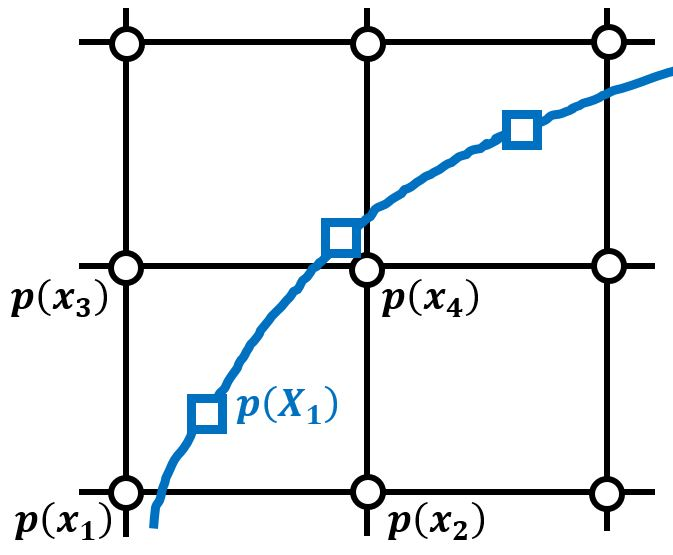
\includegraphics[width=7.00cm]{Chapter_5/figure/Chapter5_pressureMapping.jpg}
    \caption{Eulerian ($\bigcirc$) and Lagrangian ($\square$) nodes for pressure values near and on the immersed boundary.}
    \label{fig:C5_pressureMapping}
\end{figure}
%
To map this pressure information from the Eulerian nodes, $x_i$, to the Lagrangian node, $X$, we convolute the pressure field calculated from the CFD simulation with RD function of Equation \eqref{eq:C5_pressureDeltaFunction}.  By this approach we have calculated the pressure load on the structure. This is shown in Equation \eqref{eq:C5_surfacePressureCalculation}
%
\begin{subequations}
\begin{align}
    \mathcal{D}(x, X) &=
    \dfrac{-\tanh^{2}{\left (\dfrac{x - X}{\eta} \right )} + 1}{2 \eta}
    \label{eq:C5_pressureDeltaFunction}
    \\
    p(X, Y) &= \int \int p(x,y) \mathcal{D}(x, X) \mathcal{D}(y, Y) dx dy
    \label{eq:C5_surfacePressureCalculation}
\end{align}
\end{subequations}
%
By applying this pressure distribution on the solid domain and solving the equation of motion, we can calculate the displacement and the resulting velocity of the solid structure. The structure new location is used to update the RD function used for data transfer between the Eulerian and Lagrangian nodes. The cost of updating the RD functions for IB method is minuscule compared to the effort required to update the mesh in body conformal discretization approaches. The velocity of the solid domain is used for calculating the force terms required by the IB method as shown in Equation \eqref{eq:C5_immersedBoundaryForceTerm}.
%
\begin{equation}\label{eq:C5_immersedBoundaryForceTerm}
    \mathbf{f}(\mathbf{X}, t) = 
    \alpha \int_0^t \left[ \mathbf{u}(\mathbf{X}, \tau) - \mathbf{V}(\mathbf{X}, \tau) \right] d\tau + 
    \beta \left[ \mathbf{u}(\mathbf{X}, \tau) - \mathbf{V}(\mathbf{X}, \tau) \right]
\end{equation}
%
As described in Chapter \ref{ch:shapeSenwithIB}, $\mathbf{u}(\mathbf{X}, \tau)$, is the velocity of fluid calculated at the Lagrangian point $\mathbf{X}$ at time $\tau$, and $\mathbf{V}(\mathbf{X}, \tau)$ is the velocity of the solid structure at the same location and time. The later is calculated after solving the structure's equation of motion. This loop is continued until the convergence is meet or the process stoped manually. The flowchart for the fluid solid interaction using the IB method is shown in Figure \ref{fig:C5_FSIflowchart}.
%
\begin{figure}[H]
    \centering
    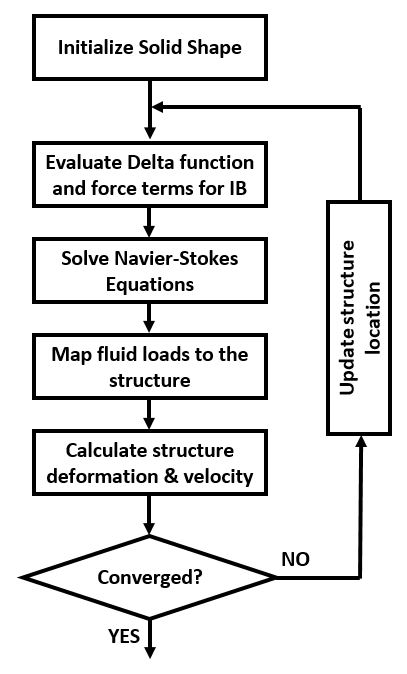
\includegraphics[width=7.00cm]{Chapter_5/figure/Chapter5_FSI_FlowChart.jpg}
    \caption{Fluid-solid interaction analysis using IB method flow chart.}
    \label{fig:C5_FSIflowchart}
\end{figure}
%
\section{Multidisciplinary Shape Sensitivity Analysis}
% =============================
The shape sensitivity analysis for the coupled multidisciplinary problem is built on the work done in Chapter \ref{ch:shapeSenwithIB}. However, in this chapter, we are also including the shape sensitivity effects on the structural side. To do so, we differentiate Equations \eqref{eq:C5_fluidGE} and \eqref{eq:C5_solidGE} alongside the kinematic and dynamic constraints of Equation \eqref{eq:C5_FSIconstraints} with respect to shape design variable, $b$. The sensitivity equations for the fluid and solid domains are shown in Equation \eqref{eq:C5_fluidSA} and \eqref{eq:C5_solidSA}, respectively.
%
\begin{subequations}\label{eq:C5_fluidSA}
\begin{align}
	&\rho^f \frac{\partial}{\partial t} \left( \frac{\partial \mathbf{u}^f}{\partial b} \right) + 
	\rho^f \frac{\partial \mathbf{u}^f}{\partial b} \cdot \nabla \mathbf{u}^f +
	\rho^f \mathbf{u}^f \cdot \nabla \left( \frac{\partial \mathbf{u}^f}{\partial b} \right) = 
	\nabla \cdot \left( \frac{\partial \mathbf{\sigma}^f}{\partial b} \right) +
	\rho^f \frac{\partial \mathbf{f}^f}{\partial b}
	\\
	&\nabla \cdot \left( \frac{\partial \mathbf{u}^f}{\partial b} \right) = 0
	\\
	&\frac{\partial \mathbf{\sigma}^f}{\partial b} = 
	\mu \left[ \nabla \left( \frac{\partial \mathbf{u}^f}{\partial b} \right) + 
	           \nabla \left( \frac{\partial \mathbf{u}^f}{\partial b} \right)^T \right] - 
	\frac{\partial p^f}{\partial b} \mathbf{I}
\end{align}
\end{subequations}
%
\begin{subequations}\label{eq:C5_solidSA}
\begin{align}
	\rho^s \frac{\partial \dot{\mathbf{u}}^s}{\partial b} &= 
	\nabla \cdot \left( \frac{\partial \sigma^s}{\partial b} \right) + 
	\frac{\partial \mathbf{f}^s}{\partial b}
	\\
	\frac{\partial \mathbf{\epsilon^s}}{\partial b} &=
	\frac{1}{2}
	\left[ \nabla \frac{\partial \mathbf{d}^s}{\partial b} + \nabla \left( \frac{\partial \mathbf{d}^s}{\partial b} \right)^T \right]
	\\
	\frac{\partial \mathbf{\sigma}^s}{\partial b} &= 
	\frac{\partial \mathbf{C}}{\partial b} : \mathbf{\epsilon}^s + 
	\mathbf{C} : \frac{\partial \mathbf{\epsilon}^s}{\partial b}
\end{align}
\end{subequations}
%
%
%\begin{subequations}\label{eq:C5_FSIconstraintsSA}
%\begin{align}
%	\frac{\partial \mathbf{u}^s}{\partial b} - 
%	\frac{\partial \mathbf{u}^f}{\partial b} &= 0
%	\\
%	\frac{\partial \mathbf{\sigma}^s}{\partial b} \cdot \mathbf{n} - 
%	\frac{\partial \mathbf{\sigma}^f}{\partial b} \cdot \mathbf{n} &= 0
%\end{align}
%\end{subequations}
\begin{subequations}\label{eq:C5_FSIconstraintsSA}
\begin{align}
	\frac{D \mathbf{u}^s}{D b} - 
	\frac{D \mathbf{u}^f}{D b} &= 0
	\\
	\frac{D \mathbf{\sigma}^s}{D b} \cdot \mathbf{n} - 
	\frac{D \mathbf{\sigma}^f}{D b} \cdot \mathbf{n} &= 0
\end{align}
\end{subequations}
%
The derivatives of the interface conditions of Equation \eqref{eq:C5_FSIconstraintsSA} are written and simplified using the chaine rule. Here we show the process for the Dirichlet boundary condition. The same approach can be done for the Neumann boudaries as well.
%
\begin{gather*}
	\overbrace{	
	\left(
	\frac{\partial \mathbf{u}^s}{\partial b} +
	\frac{\partial \mathbf{u}^s}{\partial \mathbf{x}^s} \frac{\partial \mathbf{x}^s}{\partial b} +
	\frac{\partial \mathbf{u}^s}{\partial \mathbf{x}^f} \frac{\partial \mathbf{x}^f}{\partial b}
	\right)
	}^{\dfrac{D \mathbf{u}^s}{D b}} -
	\overbrace{
	\left(
	\frac{\partial \mathbf{u}^f}{\partial b} +
	\frac{\partial \mathbf{u}^f}{\partial \mathbf{x}^s} \frac{\partial \mathbf{x}^s}{\partial b} +
	\frac{\partial \mathbf{u}^f}{\partial \mathbf{x}^f} \frac{\partial \mathbf{x}^f}{\partial b}
	\right)
	}^{\dfrac{D \mathbf{u}^f}{D b}} = 0 \Longrightarrow
	\\
	\left(
	\frac{\partial \mathbf{u}^s}{\partial b} - \frac{\partial \mathbf{u}^f}{\partial b}
	\right) +
	\left(
	\frac{\partial \mathbf{u}^s}{\partial \mathbf{x}^s} - 
	\frac{\partial \mathbf{u}^f}{\partial \mathbf{x}^s}
	\right) \frac{\partial \mathbf{x}^s}{\partial b} +
	\left(
	\frac{\partial \mathbf{u}^s}{\partial \mathbf{x}^f} - 
	\frac{\partial \mathbf{u}^f}{\partial \mathbf{x}^f}
	\right) \frac{\partial \mathbf{x}^f}{\partial b} = 
	0 \Longrightarrow
	\\
	\left(
	\frac{\partial \mathbf{u}^s}{\partial b} - \frac{\partial \mathbf{u}^f}{\partial b}
	\right) +
	\frac{\partial }{\partial \mathbf{x}^s}
	\underbrace{	
	\left(
	\mathbf{u}^s - \mathbf{u}^f
	\right)
	}_{=\mathbf{0}} \frac{\partial \mathbf{x}^s}{\partial b} +
	\frac{\partial }{\partial \mathbf{x}^f}
	\underbrace{	
	\left(
	\mathbf{u}^s - \mathbf{u}^f
	\right)
	}_{=\mathbf{0}} \frac{\partial \mathbf{x}^f}{\partial b} = 
	0 \Longrightarrow
	\\
	\frac{\partial \mathbf{u}^s}{\partial b} - 
	\frac{\partial \mathbf{u}^f}{\partial b} = 0
\end{gather*}
%
Sensitivity of solid shape movement is represented in the derivative of the forcing function, $\mathbf{f}^f$ in Equation \eqref{eq:C5_fluidSA}. In particular the geometric sensitivity of the solid boundary is added to the governing equations through the derivative of the regulirized delta function in Equation \eqref{eq:C5_fluidSA}. However, as discussed in Chapter \ref{ch:sensitivityAnalysis}, the geometric sensitivity does not propagate inside the domain since the fluid mesh does not move.

To solve the sensitivity equations we need to obtain the solution of the governing equation ($\mathbf{u}^f$, $\mathbf{\epsilon^s}$). Therefore, we are proposing to use the flowchart of Figure \ref{fig:C5_SAflowchart} for the coupled multidisciplinary sensitivity analysis. The sensitivity calculation process starts by solving the Navier-Stokes equation and mapping the pressure to the structural domain to calculate the deformation in the structural domain. The solution of the Navier-Stokes and Elasticity equations are then fed to the sensitivity solver to calculate the sensitivity response. This loop is continued until a convergence for the governing equations is reached or the process is stopped manually. 
%
\begin{figure}[H]
    \centering
    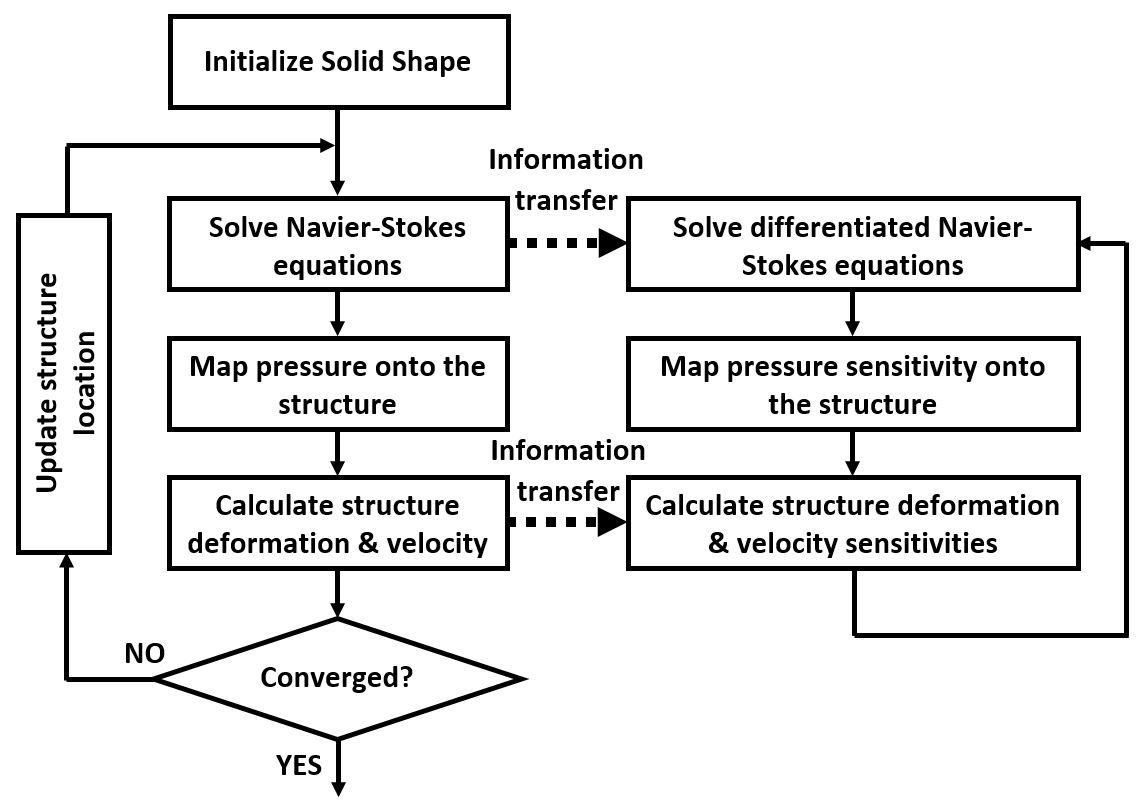
\includegraphics[width=14.00cm]{Chapter_5/figure/couple_SA_flowchart.jpg}
    \caption{Coupled multidisciplinary sensitivity analysis flowchart. The loop represents time marching for solution convergence.}
    \label{fig:C5_SAflowchart}
\end{figure}
%
\section{Problem definition}
\subsection{Governing Equations}
\subsection{FSI Coupling}
\section{Results}
\section{Summary}